\chapter{Quantifying}

The following argument is  intuitively valid.
\[ \begin{array}{p{3.5cm}}
    All people are mortal. \\
    Socrates is a person. \\ \hline Socrates is mortal. \end{array} \]
However, the validity of this argument cannot be established by the
methods we developed in the previous chapters.  In particular, in this
argument, none of the sentences is logically complex --- i.e.\ none of
them is a conjunction, or a disjunction, or a conditional, or a
negated sentence.  Hence, the proper symbolization of this argument
would be $P,Q\vdash R$.  That sequent is invalid.  Therefore the
methods of the previous chapters would lead you to say that the
argument about Socrates is invalid.  Apparently the methods of the
previous chapters get this one wrong.\footnote{For the \"uber-critical
  reader: you might translate ``all people are mortal'' as a very long
  conjunction, and then the argument would show itself to be valid.
  We would reply to your objection by presenting an argument with a
  premise about all natural numbers.}

Here's another intuitively valid argument.
\[ \begin{array}{p{6.5cm}} Professor Dumbledore believes in magic.  \\
    \hline Some professors believe in magic.  \end{array} \] Again, by
the lights of propositional logic, the premise and conclusion of this
argument are \glspl{atomic sentence}.  Hence, the argument should be
symbolized as $P\vdash Q$, which is invalid.

We are going to move forward with the assumption that the above
arguments are valid.  To see {\it why} they are valid, we need a
deeper analysis than that provided by propositional logic.  As before,
the most important clue is the appearance of certain special words and
phrases that connect the ``content words'' in the argument.  In the
first argument, the key connecting word is ``all'', as we can see by
replacing the content words (person, mortal, Socrates) with letters.
\[ \begin{array}{p{3cm}}
     All $P$ are $M$. \\
     $s$ is $P$. \\ \hline Therefore, $s$ is $M$. 
   \end{array} \]  If you replace these letters with any grammatically suitable words,
 you'll find that the result is once again a good argument.  That's a
 sign that we've identified a valid argument form.  The next step then
 is to decide how to deal with the word ``all.''  Our previous logic words
 (and, or, if\dots then, not) played the role of sentence connectives:
 they construct new sentences out of old ones.  The word ``all'' plays
 a different role.  Here it seems to transform two predicate phrases
 (``\dots is a person'' and ``\dots is mortal'') into a sentence.  It
 doesn't make any sense to think of
 ``all'' as combining these phrases
 in the same way that, say, ``and'' combines two sentences.  

To see how ``all'' works, let's take a quick detour through another
argument.  
\[ \begin{array}{p{7.5cm}}
  If Socrates is a person then Socrates is mortal. \\
  Socrates is a person. \\ \hline
  Therefore, Socrates is mortal. \end{array} \] 
This argument {\it is} valid in respect to its propositional form
-- it's just an instance of modus ponens.  However, propositional
logic would have us use two completely different letters for
``Socrates is a person'' and ``Socrates is mortal'', thereby losing
track of the fact that those two sentences have the same subject.  So
now let's write $Ps$ for ``Socrates is a person'', and $Ms$ for
``Socrates is mortal''.  Then the argument would be symbolized as:
\[ \begin{array}{l}
Ps\to Ms \\
Ps \\ \hline 
Ms \end{array} \] 
Keeping your eye on the first premise $Ps\to Ms$, return now to the
question of how to represent the logical form of ``all persons are mortal.''
Let's remove the name Socrates, and replace it with a
place holder.  We'll use the letter ``$x$'' as our place holder.  Then
we get ``if $x$ is a person, then $x$ is mortal'' ($Px\to Mx$), which isn't exactly
a sentence, but which can be used to create sentences by plugging a
name in for $x$.  If we plug in $s$, we get the sentence $Ps\to Ms$.
Now, the sentence ``all $P$ are $M$'' says that no matter what name we
plug in for $x$, the resulting sentence is true, i.e.\ $Pa\to Ma$ is
true, and $Pb\to Mb$ is true, etc.  Thus, the first premise of our
original Socrates argument can be partially symbolized as:
\[ \begin{array}{p{8cm}}
     For any $x\:$ $(Px\to Mx)$ \end{array} \]
Now let's replace ``For any $x$'' with a symbol $\forall x$, yielding
the following symbolization of the original argument.
\[ \begin{array}{l}
     \forall x(Px\to Mx) \\
     Ps \\ \hline Ms \end{array} \] This argument form is valid, and we might want to add it as a
 basic rule.  But that would be a little short-sighted, because it
 wouldn't capture the full logical power of the concept represented by
 $\forall x$.  For example, the following argument form is also valid:
 \[ \begin{array}{l} \forall x(Fx\wedge Gx) \\ \hline \forall
     xFx \end{array} \] That is, if everything is both $F$ and $G$,
 then everything is $F$.  That's another obviously valid argument,
 indicating that $\forall x$ occurs in many different valid argument
 forms.  Our goal is to find the most basic valid inferences using
 $\forall x$, and then to show that these intuitively valid arguments
 -- and all others -- can be reconstructed from those basic valid
 inferences.

The newly introduced symbol $\forall x$ will be called the
\gls{universal quantifier}.  We used symbol $x$ as our placeholder,
and will call it a \gls{variable}, but that doesn't mean that any
``varying'' is happening here.  It's just a symbol.  We will also
sometimes use other letters at the end of the alphabet for variables,
and it will be important sometimes to have more than one variable in
play.  Suppose for example you want to represent the following
intuitively valid argument:
\[ \begin{array}{p{8cm}} 
  $\forall x$($\,x$ is divisible by $a$ $\,\to\,$ $x$ is divisible by $b\,$) \\
     $c$ is divisible by $a$ \\ \hline
     $c$ is divisible by $b$
   \end{array} \]
Here ``$x$ is divisible by $y$'' is a relation that holds between two
things, rather than a property of a single thing.  To represent ``$x$
is divisible by $y$,'' we can use a symbol such as $Dxy$ that has two
variables.  Then we can represent the preceding argument as follows:
\[ \begin{array}{l}
     \forall x(Dxa\to Dxb) \\
     Dca \\ \hline Dcb \end{array} \] We will also need our inference
 rules for $\forall x$ to explain why this argument is valid.  But before we get to that, we need to discuss another special logical notion that plays a key role in many valid arguments.

The following argument is intuitively valid.
\[ \begin{array}{p{6cm}}
     All Harvard graduates are hilarious.  \\
     Some Harvard graduates are felons.  \\ \hline
     Some felons are hilarious.  \end{array} \]
Here the first premise is again a universally quantified
  sentence.  But the second premise and the conclusion don't say that
{\it all} things have some feature; instead, they say that {\it some}
things have that feature.  We introduce a new symbol $\exists$
corresponding to the phrase ``There are some \dots '', and hence we
symbolize ``There are some things with feature $F$'' as $\exists
xFx$.  In the second premise we say that there are things that are
both Harvard graduates ($Hx$) and felons ($Fx$); hence it could be
symbolized as $\exists x(Hx\wedge Fx)$.  

The symbol $\exists x$ is called the \gls{existential quantifier}
because it expresses that something exists.  Like its universal
brother, it's always used with some particular variable which connects
it to the predicate or relation symbols that follow it.  Read somewhat
literally, $\exists xFx$ says that ``There is an $x$ such that $Fx$.''
Similarly, $\exists x(Fx\wedge Gx)$ says that ``There is an $x$ such
that $Fx$ and $Gx$.''

In English we have many phrases that express that something of a
certain sort exists.  We can say, ``there is \dots '' or ``there are
some \dots '' or ``something is \dots '', and many more like those.
In specific conversational contexts, these phrases can have more
specific implications --- e.g.\ they can indicate that there is more
than one, or that there are some things with this feature and some
things without it.  Consider, for example, if somebody asked your
logic professor ``do you have good students?''  If he answered, ``some
of them are good,'' then his interlocutor would reasonably conclude
that, in addition, some of them are not good.  That's because we are
often expected to answer by making the (logically) strongest statement
that we would be warranted in asserting.  If, in fact, your professor
believes that all his students are good, then why wouldn't he have
said that?

Similarly, suppose that your professor believes that only one student
in his class (of say $280$ students) is good, and that the rest of
them are terrible.  If he then says that ``some of my students are
good,'' one might justly accuse him of concealing the true situation.
He could just as easily say, ``strangely, only one of them is good.''
So, in that case, the phrase ``some'' wouldn't supply the most
accurate answer to the question.

Nonetheless, in symbolic logic, the existential quantifier has no
nuanced connotations.  The sentence ``$\exists xFx$'' simply means
that there is at least one $F$.  That's consistent with there being
only one $F$, or there being forty two $F$s, or with everything being
$F$.  If you wish that symbolic logic could be more nuanced, just
remember that what it loses in nuance it gains in clarity and rigor.

We've seen so far that we can express ``there is an $F$'' with
$\exists xFx$, and we can express ``some $F$ are $G$'' with
$\exists x(Fx\wedge Gx)$.  In a similar fashion, we can express ``some
$F$ are not $G$'' by $\exists x(Fx\wedge\neg Gx)$.  For example, to
say ``some Wall Street bankers are not evil,'' we could write
$\exists x(Wx\wedge\neg Ex)$.  Combining the expressive power of the
existential quantifier with that of the universal quantifier, we can
express the four standard sentence types that you might have seen
before in reference to Venn diagrams (Figure \ref{venn}).

\def\firstcircle{(1.5,0) circle (0.6cm)}
\def\secondcircle{(1.5,0) circle (1cm)}

\colorlet{circle edge}{black}
\colorlet{circle area}{gray!20}

\tikzset{filled/.style={fill=circle area, draw=circle edge, thick}, outline/.style={draw=circle edge, thick}}

\begin{figure}[h] \label{venn} \caption{The four standard types of quantified statements}
\centering
% Set A and B

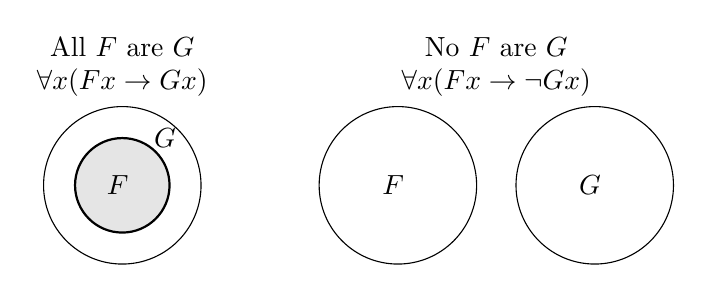
\begin{tikzpicture}[every text node part/.style={align=center}]
\draw[filled] \firstcircle node { $F$ };
\draw \secondcircle node { };
\node[anchor=south,rectangle] at (current bounding box.north) { All $F$ are $G$ \\ $\forall x(Fx\to Gx)$};
\node at (2.1,0.6) { $G$ };
% \draw (-2.5,-2.5) rectangle (4.5,2.5) node [text=black,above] {$\emptyset$};
\draw (5,0) circle (1cm) node { $F$ };
\draw (7.5,0) circle (1cm) node { $G$ };
\node[anchor=south,rectangle] at (6.25,1) { No $F$ are $G$ \\ $\forall x(Fx\to \neg Gx)$};
\end{tikzpicture}
\end{figure}

\begin{figure}
\centering
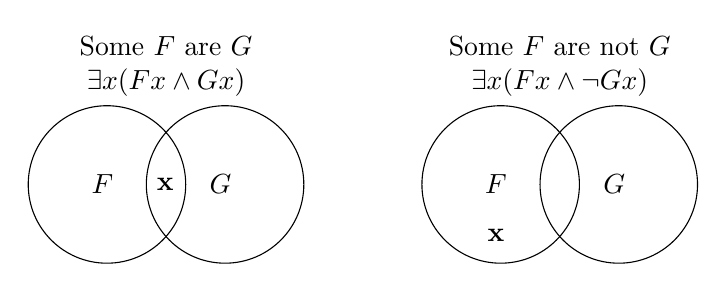
\begin{tikzpicture}[every text node part/.style={align=center}]
\draw (0,0) circle (1cm) node { $F$ };
\draw (1.5,0) circle (1cm) node { $G$ };
\draw (0.8,0) node { \textbf{x} };
\node[anchor=south,rectangle] at (0.75,1) { Some $F$ are $G$ \\ $\exists x(Fx\wedge Gx)$};
\draw (5,0) circle (1cm) node { $F$ };
\draw (6.5,0) circle (1cm) node { $G$ };
\draw (5,-0.65) node { \textbf{x} };
\node[anchor=south,rectangle] at (5.75,1) { Some $F$ are not $G$ \\ $\exists x(Fx\wedge \neg Gx)$};
\end{tikzpicture}
\end{figure}
                                                    

                                                    
                                                    
A common mistake that many beginning logic students make is to use $\exists x(Fx\to
Gx)$ for ``some $F$ are $G$''.  But a moment's thought shows that the
former symbolic sentence would be a bad translation.  The formula
$Fx\to Gx$ can be true of an individual $a$ for two different reasons.
First, $Fa\to Ga$ would be true if $Fa$ and $Ga$ are true.  But $Fa\to
Ga$ would also be true if $Fa$ were false.  (Just remember negative
paradox, or the truth-table for the conditional.)  Thus, $\exists
x(Fx\to Gx)$ would be true whenever something is not $F$, which fails
to capture the intent to assert the existence of something that is
both $F$ and $G$.

Similarly, it's easy to mistakenly write $\forall x(Fx\wedge Gx)$ when
you mean to say that ``all $F$ are $G$''.  But the sentence
$\forall x(Fx\wedge Gx)$ is way too strong: it says that everything
whatsoever is {\it both} $F$ {\it and} $G$.  Yes, it implies that all
$F$ are $G$, but only for the trivial reason that everything has both
features.  

As a general rule of thumb, if a natural language sentence is
translated to a universally quantified sentence, then the formula
inside the quantifier will be a conditional.  In contrast, if a
natural language sentence is translated to an existentially quantified
sentence, then the formula inside the quantifier will be a
conjunction.

%% exercises

\begin{exercise} Represent the form of the following sentences in
  predicate logic.  We've suggested appropriate symbols.  (For the
  sentences about people, you don't need to add an extra predicate for
  ``$x$ is a person.'')
  \begin{enumerate}
  \item No logicians are celebrities.  ($Lx,Cx$)
  \item Some celebrities are not logicians. ($Lx,Cx$)
  \item Only students who do the homework will learn logic.
    ($Sx,Hx,Lx$)
  \item All rich logicians are computer scientists. ($Rx,Lx,Cx$)
  \item All students and professors get a discount. ($Sx,Px,Dx$)
  \item No logician is rich, unless she is a computer
    scientist. ($Lx,Rx,Cx$)
  \item Not all logicians are computer scientist.  ($Lx,Cx$)
  \item Some logicians are rich computer scientists.  ($Lx,Rx,Cx$)
  \item If there are rich logicians, then some logicians are computer
    scientists. ($Rx,Lx,Cx$)
  \item No pets except service animals are permitted in dorms. ($Px,Sx,Dx$)
  \item If anyone is rich, then Mary is.  ($Rx,m$)
  \end{enumerate}
\end{exercise}

When you're symbolizing sentences, there will occasionally be cases
where there seem to be two (or more) possible correct answers.
Consider, for example, the sentence ``There are no friendly cats.''
If we use $Fx$ for ``$x$ is friendly'' and $Cx$ for ``$x$ is a cat'',
then any one of the following is a plausible representation of this
sentence:
\[ \neg\exists x(Fx\wedge Cx) \qquad \forall x(Fx\to \neg Cx) \qquad
  \forall x(Cx\to\neg Fx) \] The first sentence says that it's false
that there is a friendly cat.  The second sentence says that every
friendly thing is not a cat.  The third sentence says that every cat
is not friendly.  In English, these three statements have slightly
different connotations, and yet they would be true in precisely the
same circumstance, viz.\ the circumstance when the class of friendly
things does not include any cats.  Not long from now, you'll be able
to prove that these three sentences are in fact logically equivalent.

There are other cases where a natural language sentence is simply
ambiguous between two different ways that we might construe it in
symbolic language.  Consider, for example, the following
sentence:\footnote{This example was concocted by the logician Peter
  Geach (1916--2013).}
\begin{quote} Every boy loves a certain girl. \end{quote} Translating
this sentence might seem straightforward.  First, the sentence says
that every boy has a certain property, hence
$\forall x(Bx\to \phi (x))$, where $\phi (x)$ expresses ``$x$ loves a
certain girl''.  For the latter, we could write
$\phi (x)\equiv\exists y (Gy\wedge Lxy)$, which says that ``there is a
girl whom $x$ loves''.  The final answer then would be
\[ \forall x(Bx\to \exists yLxy ) .\] However, there's another way to
interpret this sentence: it might mean that there is some one girl who
is loved by every boy.  In that case, we want to approach the sentence
the other way around, i.e.\ we write $\exists y(Gy\wedge \psi (y))$,
where $\psi (y)$ expresses ``every boy loves $y$''.  Thus,
$\psi (y)\equiv \forall x(Bx\to Lxy)$, and the final answer is
\[ \exists y(Gy\wedge \forall x(Bx\to Lxy)) .\] Unlike the previous
example where the different translations were equivalent, these two
symbolic sentences are inequivalent --- they represent genuine
ambiguity in the initial English sentence.  In particular, it's
possible for the first sentence to be true while the second sentence
is false.\footnote{While it's intuitively clear that the first
  sentence does not imply the second, you'll first learn to prove that
  in Chapter \ref{inter}.}

The preceding considerations show that, in general, it makes a
difference which order you write quantifiers.  In fact, a famous
philosophical debate turns precisely on this point.  Among the many
attempts to prove God's existence, the so-called cosmological argument
begins from the premise that every event has a cause.  It then
concludes that there must be a first cause (which, the arguer
suggests, we can call ``God'').  If we were to try to capture the
argument in symbolic logic, then we might write the premise as
$\forall x\exists yRyx$, where $Ryx$ means that ``$y$ causes $x$''.
In that case, the conclusion would be represented as
$\exists y\forall xRyx$.  However, the philosopher Bertrand Russell
pointed out that the inference
$\forall x\exists yRyx\vdash \exists y\forall xRyx$ is {\it not}
valid.\footnote{The Russell-Copleston debate of 1948.  An audio
  recording of the debate can be found on the internet.}  Indeed, if
it were valid, then it would remain so no matter how we interpreted
the symbol $Ryx$.  But if we interpret $Ryx$ to mean that ``$y$ is the
mother of $x$'', then the premise is true of mammals, whereas the
conclusion is most definitely not true of mammals.

%% TO DO: introduce relation symbols

\begin{exercises} Represent the form of the following sentences in
  predicate logic.  We've suggested appropriate symbols.  (For the
  sentences about people, you don't need to add an extra predicate for
  ``$x$ is a person''.)
  \begin{enumerate}
  \item Mary loves everyone who loves her. ($m,Lxy$)
  \item Mary loves all and only those people who don't love
    themselves. ($Lxy,m$)
  \item Everyone loves their mother.  ($Lxy,Mxy$)
  \item Some people love only those people who love their
    mother. ($Lxy,Mxy$)
   \item Snape killed someone. ($Kxy,s$)
  \item Snape is a killer.  ($Kxy,s$)  
  \item Someone was killed by Snape. ($Kxy,s$)
  \item Some wizards only marry other wizards.  ($Wx,Mxy$) 
  \item There is no greatest number. ($Nx,x<y$)
  \item $c$ is the least upper bound of $a$ and $b$.  ($a,b,c,x\leq y$)
  \item $c$ is the greatest common divisor of $a$ and $b$.
    ($a,b,c,Dxy,x\leq y$)
   \end{enumerate} \end{exercises}


\section*{Universal Elimination}

We gave a big hint above about the meaning of $\forall x$.  We said
that somebody who accepts $\forall x\phi (x)$ would be willing to
grant that $\phi (a)$, no matter what $a$ names.  If that's right,
then the first and most obvious inference rule for quantified
statements should look like this:
\begin{quote} From $\forall x\phi (x)$, it's permitted to infer
  $\phi (a)$, for any name $a$. \end{quote} This rule will be called
\emph{universal elimination (UE)} since it permits us to infer
something from a universally quantified sentence.  Here we used the
notation $\phi (x)$ to stand for any formula that contains the
variable $x$.  For example, $\phi (x)$ could be $Px\to Mx$, or it
could be $Px\to Ms$, or it could be $Rx$.

The UE rule can be applied to prove $Ms$ from the conjunction of
$\forall x(Px\to Mx)$ and $Ps$.
\[ \begin{array}{l l >{$}p{3cm}<{$} p{1.5cm}}
  1 & (1) & \forall x(Px\to Mx) & A \\
  2 & (2) & Ps & A \\
  1 & (3) & Ps\to Ms & 1 UE \\
  1,2 & (4) & Ms & 3,2 MP \end{array} \]
Universal elimination (UE) is one of those simple rules of inference
where we carry down the dependency numbers of the sentence we use.  In
the above argument, we apply UE to line 1, which depends only on
itself.  Thus, the resulting line, i.e.\ line 3, also depends on just
line 1.

Here's the precise formulation of the UE rule.
\bigskip \begin{tcolorbox}[enhanced,width=10cm,title=Universal Elimination (UE),attach boxed title to top
  left={yshift=-2mm,xshift=4mm},boxed title style={sharp corners}]
From a universal sentence, you can infer any instance.  Schematically:  
$\begin{array}{l l}
     \Gamma\:\vdash\:\forall x\phi (x) \\
     \hline
     \Gamma\:\vdash\:\phi (a) \end{array} $
\end{tcolorbox} \bigskip

%% Now UE exercises

\begin{exercises} Prove the following sequents.
\begin{enumerate}
\item $\forall xFx,\forall xGx\:\vdash\: Fa\wedge Ga$
\item $\forall x\neg Fx\:\vdash\: Fa\to P$
\item $\forall x(Fx\to Gx),\neg Ga\:\vdash\:\neg Fa$
\item $\forall x(Fx\to Gx),\neg Ga\:\vdash\:\neg \forall xFx$  
\item $\forall x\neg Fx\:\vdash\:\neg\forall xFx$
\item $\vdash\:\neg\forall x(Fx\wedge\neg Fx)$
\end{enumerate}
\end{exercises}

\begin{exercise} Do the sentences $\forall x(Fx\to Gx)$ and
  $\forall x(Fx\to \neg Gx)$ seem consistent to you? \end{exercise}



\section*{Universal Introduction}

The UE rule won't do much for you on its own.  For example, if you're
trying to infer $\forall xFx$ from $\forall x(Fx\wedge Gx)$, UE can
take you down to $Fa\wedge Ga$, but it can't get you back up to
$\forall xFx$.  Indeed, to infer a universal sentence from any
particular instance is the worst kind of mistake.  For example, you
cannot conclude that all professors believe in magic from the fact
that Professor Dumbledore believes in magic.  Thus, in order to get
the most out of the UE rule, it needs to be supplemented with a
universal introduction rule.

Recall that conditional proof isn't just a rule, it's a strategy for
thinking.  In short, if you want to prove a conditional, then your
first move is to assume the antecedent, which you can use in reasoning
toward the consequent.  Now, universal introduction (UI) will be like
conditional proof in this regard.  Only now we have to think about
how we come to be convinced of the truth of universal statements.

It is really quite amazing that human beings can ever come to know
that a universal statement is true.  We are limited in space and time,
and none of us will ever be able to survey all possible instances of
any generalization.  So what could permit us -- who can only observe
a small finite number of instances -- to conclude that something is
always true?

The answer is similar to the one we gave for conditional statements.
To reason to a conditional statement, we engage in the mental activity
of {\it supposing}, an activity that is not itself aimed at telling
the truth.  When I say ``suppose that $P$,'' I am not making a claim
about what is the case; instead, I'm abstracting away from reality so
that I can explore logical connections.  When it comes to
establishing universal claims, we engage in an even more radical
version of abstraction.  In essence, we suppose that we can talk about
things in general, without talking about any particular thing.

Consider the following dialogue where A and B agree that all Bavarians
are German, and all Germans are European, and A is trying to convince
B that all Bavarians are European.

\begin{quote} A: Suppose that Gretel is some random Bavarian. \newline
  B: So the random Bavarian is female?  \newline
  A: No, I didn't mean that at all.  I just meant to choose a
  Bavarian-sounding name.  If I had chosen ``Hansel,'' you might have
  asked me if the random Bavarian is male. \newline
  B: Why don't you just use a letter then? \newline
  A: OK, suppose that $X$ is some random Bavarian.  
  You agree with me then that $X$ is German, right?  \newline
  B: Yes, certainly.  \newline
  A: And since all Germans are European, $X$ is European.
  \newline
  B: Agreed. \newline
  A: Since $X$ was an arbitrary Bavarian, it follows that every Bavarian is European.  \end{quote}

It's this last step where all the action happens.  The letter $X$
plays the role of name, but we don't know anything about who it names
-- except that he or she is Bavarian.  So, when we deduce that $X$ is
European, that licenses us to conclude that {\it all} Bavarians are
Europeans.

We have to beware of a danger here.  In the above dialogue, the two
parties chose the letter $X$ because there was little danger that the
letter would carry connotations that would derail their reasoning
process.  But there are no guarantees.  What if B were obtuse, like this.
\begin{quote}
  B: Since the arbitrary Bavarian's name is ``$X$'', it follows that no
  Bavarians have the name ``Gretel.'' \end{quote} Obviously, something
has gone very wrong with B's thinking about these issues.
Essentially, B forgot that the whole point of choosing a letter ``$X$''
was so that nobody would assume they know anything about $X$.  But
that's exactly what B has done, she has assumed that $X$ has the
feature that its name is ``$X$''.  She has missed the point
completely.

In real-life reasoning, people have common sense to prevent them from
making such mistakes.  But the goal of formal logic is to make
explicit the rules that common sense suggests.  We want to forbid this
kind of mistake by means of an explicit rule, and here's how we'll do
it.

To use an analogy, suppose that the argument or dialogue takes place
in a closed room.  And suppose that when the two parties enter the
room, they each have to declare their assumptions.  Once the dialogue
begins, they can use those assumptions that they declared upon
entering the room.  When it comes to reasoning about universal claims,
we'll give both parties a stock of new names $a,b,c,\dots $, that do
{\it not} occur anywhere in their declared assumptions.  They may then
use these names at any point in their argument.  For example, they may
use UE to infer $\phi (a)$ from $\forall x\phi (x)$.

With these new regulations in place, we can prevent the parties from
making silly mistakes in deducing universal sentences.  In short, one
may infer a universal sentence $\forall x\phi (x)$ from an instance
$\phi (a)$ that contains one of the new names we supplied.  Since the
two parties didn't bring in any information about $a$, the only
information they can have about $a$ is what they have deduced from
universal statements.

Hopefully the analogy helps your intuition.  But you won't need the
intuition to follow the universal introduction rule, which provides a
simple (machine checkable!) syntactic recipe.  In short, UI allows you
to infer $\Gamma\vdash\forall x\phi (x)$ from $\Gamma\vdash \phi (a)$
whenever there is no information about $a$ in the background
assumptions $\Gamma$, or hidden in the formula $\phi (x)$.

\bigskip \begin{tcolorbox}[enhanced,width=10cm,title=Universal Introduction (UI),attach boxed title to top
  left={yshift=-2mm,xshift=4mm},boxed title style={sharp corners}]
\[ \begin{array}{r@{\; }c@{\; }l c@{\quad }p{6cm}}
       \Gamma & \vdash & \phi (a) & & \multirow{2}{6cm}{\small restriction: $a$ does not occur in $\Gamma$ or $\phi (x)$.} \\ \cline{1-3}
       \Gamma & \vdash & \forall x\phi (x) \end{array} \]  
 \end{tcolorbox} \smallskip

In general, universally quantified premises can be used together to
draw universally quantified conclusions.  The strategy is often as
simple as applying UE repeatedly to the premises, making sure to use
the same name in each case.  Then one uses the rules of propositional
logic to transform those instances to an instance of the conclusion.
Finally, one applies UI to infer the conclusion from that instance.

\medskip \noindent \textbf{To prove:} $\forall x(Fx\to Gx),\forall x(Gx\to Hx)\:\vdash\: \forall x(Fx\to Hx)$
\[ \begin{array}{l l >{$}p{3.5cm}<{$} p{2cm}}
     1 & (1) & \forall x(Fx\to Gx) & A \\
     2 & (2) & \forall x(Gx\to Hx) & A \\
     3 & (3) & Fa                  & A \\
     1 & (4) & Fa\to Ga            & 1 UE \\
     2 & (5) & Ga\to Ha            & 2 UE \\
     1,3 & (6) & Ga                & 4,3 MP \\
     1,2,3 & (7) & Ha              & 5,6 MP \\
     1,2 & (8) & Fa\to Ha          & 3,7 CP \\
     1,2 & (9) & \forall x(Fx\to Hx) & 8 UI \end{array} \] Looking at
 the conclusion, we realized that we need to show that an arbitrary $F$ is also an $H$.  That is, we need to show that $Fa\to Ha$, depending on no assumptions that mention $a$.  So then on line 3, we suppose that $a$ is an arbitrary $F$.  (There is nothing in line 3 that says ``is an arbitrary,'' but that effect is ensured by choosing a name $a$ that hasn't yet occurred in the proof.)  Then we proceed to use the universal premises to infer that $a$ is also an $H$.
 
 The restriction on the name $a$ corresponds to the idea that a fully
 general statement cannot be inferred from specific assumptions.  To
 see why we prohibit $a$ from occurring in $\phi (x)$, consider the
 following attempt to prove $\forall xRxa$ from $\forall xRxx$.
\[ \begin{array}{l l >{$}p{2cm}<{$} p{1cm} p{4cm}}
     1 & (1) & \forall xRxx & A \\
     1 & (2) & Raa          & 1 UE \\
     1 & (3) & \forall xRxa & 2 UI &
                                     $\Longleftarrow$
                                     incorrect \end{array} \] %
This argument cannot possibly be valid.  Suppose that $Rxy$ is the
relation ``$x$ has the same net worth as $y$'' and that $a$ is a name
for Jeff Bezos.  The premise is then obviously true: everybody has the
same net worth as themselves.  But the conclusion says that everyone
has the same net worth as Jeff Bezos, which is as far from the truth
as possible.  The problem here is line 3, since the formula $\phi (x)$
is $Rxa$, which contains the name $a$.  In practice, you can ensure
that you don't violate this restriction on UI if you follow this rule
of thumb: when generalizing $\phi (a)$ to $\forall x\phi (x)$, 
change all occurrences of $a$ to $x$. In the case at hand, that would
have forced us to generalize $Raa$ to $\forall xRxx$, which is just
what we started with.

% When you're trying to derive a universal conditional such as
% $\forall x(Fx\to Gx)$, then it makes sense to begin by assuming $Fa$,
% where $a$ is a new name.  You can then apply UE to any universal
% premises to try to get information that will allow you to derive $Ga$.
% In other cases, it makes sense just to start by applying UE to your
% premises, to see if they give you the conclusion you want.  For
% example, in the following proof, we need to show that an arbitrary
% thing if $F$.  For that, it would suffice to show that $Fa$ for an
% arbitrary $a$; and applying UE to line 1 yields $Fa\wedge Ga$.
% \[ \begin{array}{l l >{$}p{2.5cm}<{$} p{1.5cm}}
%      1 & (1) & \forall x(Fx\wedge Gx) & A \\
%      1 & (2) & Fa\wedge Ga & 1 UE \\
%      1 & (3) & Fa & 2 $\wedge$E \\
%      1 & (4) & \forall xFx & 3 UI \end{array} \] The use of UI on line
% 4 is permitted because line 3 depends only on 1, and the name $a$ does not occur in line 1.

%% TO DO: slightly more interesting use of UI

The UI rule can be used with any variable.  For example, $\phi (a)$
can be quantified to $\forall x\phi (x)$ or $\forall y\phi (y)$ or
$\forall z\phi (z)$.  You only need to make sure not to get yourself
confused by using a variable that already occurs in $\phi (a)$.  So,
for example, you wouldn't infer $\forall x\forall xRxx$ from
$\forall xRax$, because the former string of symbols doesn't make
sense as a formula.

Using the freedom to apply UI with any variable, it follows that
universal statements $\forall xFx$ and $\forall yFy$ are equivalent.
\[ \begin{array}{l l >{$}p{2.5cm}<{$} p{2cm}}
     1 & (1) & \forall xFx & A\\
     1 & (2) & Fa          & 1 UE \\
     1 & (3) & \forall yFy & 2 UI \end{array} \] The converse proof
 follows by symmetry, hence $\forall xFx\dashv\vdash \forall yFy$.
 These equivalences -- where one variable is switched throughout for
 another -- are known as $\alpha$-equivalences, and they can be really
 useful when dealing with sentences that contain more than one
 variable.  For example, by $\alpha$-equivalence, $\forall xFx\to
 \forall yFy$ is a tautology; and we'll soon see that $\forall xFx\to
 P$ implies $\exists x(Fx\to P)$.  Thus, substituting $\forall
 yFy$ for $P$ shows that $\exists x(Fx\to \forall yFy)$ is a tautology.

\begin{exercises} Prove the following sequents. \label{ex:ui}
  \begin{enumerate}
    \item $\forall x(Fx\to Gx)\:\vdash\: \forall xFx\to \forall xGx$
    \item $\forall x(Fx\to Gx)\:\vdash\:\forall x\neg Gx\to \forall
      x\neg Fx$
    \item $\forall xFx\wedge \forall xGx\:\dashv\vdash\: \forall x(Fx\wedge
      Gx)$
    \item $\forall xFx\vee \forall xGx\:\vdash\: \forall x(Fx\vee Gx)$
    \item $\neg Fa\:\vdash\:\neg\forall xFx$
    \item $\forall x\neg Fx\:\vdash\:\forall x(Fx\to Gx)$
    \item $P\:\vdash\: \forall x(Fx\to P)$, where $P$ is any sentence
      that doesn't contain the variable $x$.
    \item $P\to \forall xFx\:\dashv\vdash\: \forall x(P\to Fx)$  
    \item $\forall x\forall yRxy\:\vdash\: \forall xRxx$
    \item $\forall x\forall yRxy\:\vdash\: \forall y\forall xRxy$
    \end{enumerate}
  \end{exercises}

  \begin{exercise} What's wrong with the following attempted proof? 
\[ \begin{array}{l l >{$}p{3cm}<{$} p{1.5cm}}
     1 & (1) & Fa  & A \\
       & (2) & Fa\to Fa & 1,1 CP \\
       & (3) & \forall x(Fa\to Fx) & 2 UI  \\
       & (4) & Fa\to Fb & 3 UE \end{array} \] \end{exercise}

 \begin{exercise} Start to try to write a proof of \[ \forall x(Fx\vee
  Gx)\:\vdash\:\forall xFx\vee \forall xGx ,\] and explain where the
  restriction on UI prevents you from continuing. \end{exercise}  
  

\section*{Existential Introduction}

It's not too uncommon that we know that there is something or other
with a certain feature, but we don't know who or what it is that has
that feature.  For example, we know that somebody murdered eleven
women in London in the years 1888 to 1891, but as of today, the
identity of the murderer is still unknown.

We can also use such knowledge to infer other things, although we have
to be careful when using knowledge that ``something is $\phi$''
without knowing who or what it is that is $\phi$.  For example, if you
know that something is $\phi$, and you know that all $\phi$ are
$\psi$, then you also know that something is $\psi$.  In contrast, you
might know that something is $\phi$ and that something is $\psi$; but
those two facts do {\it not} entitle you to conclude that something is
both $\phi$ and $\psi$.

What then is the logic of ``something is $\phi$''?  As with our other
key logical notions, we are looking here for typical inferences to
such statements (an introduction rule), and typical inferences
from such statements (an elimination rule).

Let's look first for an existential intro rule -- i.e.\ a paradigmatic
inference to a statement of the form ``something is $\phi$.''  In real
life, our reasons for believing existential statements are frequently
not {\it guaranteeing} reasons, in the sense that the existential
statement is a logical consequence of what we know.  For example, in
the Jack the Ripper case, the reason that I believe that somebody
killed eleven women is because I read about it, or heard about it on
TV.  But of course, the documentary evidence doesn't guarantee -- in a
logical sense -- that the event actually happened.  So this kind of
evidence is not what we're looking for in a deductively valid rule of
existential introduction.

However, there was at least one person who had guaranteeing evidence
for the claim that someone killed eleven women.  In particular, Jack
the Ripper -- if he existed -- knew that ``I killed eleven women,''
and so he would have been entitled to infer that ``somebody killed
eleven women.''  There is {\it no way} that the premise could be true
and the conclusion false, indicating the presence of a valid argument
form.  Thus, Jack the Ripper's valid inference could be represented as
follows:
\[ \begin{array}{c} \phi (a) \\ \hline \exists x\phi
    (x) \end{array} \] Here $a$ is Jack's name for himself, and
$\phi (x)$ represents ``$x$ murdered eleven women.''  Thus, the
inference goes from ``I murdered eleven women'' to ``somebody murdered
eleven women.''  We'll take this inference to be the paradigm way that
an existential statement can be inferred from another statement.
\bigskip \begin{tcolorbox}[enhanced,width=10cm,title=Existential
  Introduction (EI),attach boxed title to top
  left={yshift=-2mm,xshift=4mm},boxed title style={sharp corners}] If
  an instance $\phi (a)$ of $\exists x\phi (x)$ follows from $\Gamma$,
  then $\exists x\phi (x)$ follows from $\Gamma$.  Schematically:
$\arraycolsep=1.4pt \begin{array}{r c l}     \Gamma & \vdash & \phi (a) \\
     \hline
     \Gamma & \vdash & \exists x\phi (x) \end{array} $
\end{tcolorbox} \bigskip
\noindent Here $\phi (x)$ is a formula in which the variable $x$ occurs, and
$\phi (a)$ is the formula that is obtained by replacing all the
instances of $x$ in $\phi (x)$ with $a$.  However, there is no requirement that $a$ does
{\it not} occur in $\phi (x)$.  For example, it's perfectly legitimate
to infer that somebody killed Ernest Hemingway from the fact that
Ernest Hemingway committed suicide.  That is, $\exists xKxa$ can be
inferred, by existential intro, from $Kaa$.  

Like disjunction intro, existential intro actually throws away
information -- and so it's dangerous to use it without knowing where
you want to go.  Remember that disjunction intro is most useful in
cases where you want to show that two different premises have the same
conclusion.  We'll soon see that the same sort of intuition applies to
existential intro, i.e.\ it's most effective in the search for a
common conclusion from several different premises. 

Nonetheless, there are some cases where EI by itself is useful.  In
the following we show that a negated existential sentence implies a
universal sentence. \label{qne}

\medskip\noindent\textbf{To prove:} $\neg\exists xFx\vdash\forall x\neg Fx$
\[ \begin{array}{l l >{$}p{4cm}<{$} p{2cm}}
     1 & (1) & \neg\exists xFx & A \\
     2 & (2) & Fa              & A \\
     2 & (3) & \exists xFx     & 2 EI \\
     1,2 & (4) & \exists xFx\wedge\neg\exists xFx & 3,1 $\wedge$I \\
     1   & (5) & \neg Fa     & 2,4 RAA \\
     1   & (6) & \forall x\neg Fx  & 5 UI \end{array} \]
(Note that since line 5 depends only on line 1, and line 1 does not
contain $a$, the invocation of UI on line 6 is legitimate.)  Here our
strategy is not completely straightforward.  The premise $\neg\exists
xFx$ is not in itself useful: it's a negated sentence, and none of our
rules will let us do something with a single negated sentence.  We
then have to work our way backwards from the conclusion, which is
$\forall x\neg Fx$.  Since it's a universal sentence, it would suffice
to obtain an instance $\neg Fa$, so long as that instance doesn't
depend on any assumptions about $a$.  In frustration, one might decide
(as we did) to try to obtain $\neg Fa$ by reductio ad absurdum.
Indeed, as soon as we assumed $Fa$, it was obvious that it conflicts
with the premise on line $1$.

Notice that if we run through the preceding proof, replacing $Fx$ with
$\neg Fx$, then line 5 would become $\neg\neg Fa$.  We can then perform a
step of DN elimination to get $Fa$, and then $\forall xFx$.  Thus, we also
have a proof of the sequent $\neg\exists x\neg Fx\vdash\forall xFx$.

% \[ \begin{array}{l l >{$}p{4cm}<{$} p{2cm}}
%      1 & (1) & \neg\exists x\neg Fx & A \\
%      2 & (2) & \neg Fa              & A \\
%      2 & (3) & \exists x\neg Fx     & 2 EI \\
%      1,2 & (4) & \exists x\neg Fx\wedge \neg\exists x\neg Fx & 3,1
%                                                                $\wedge$I
%      \\
%      1 & (5) & \neg\neg Fa  & 2,4 RAA \\
%      1 & (6) & Fa           & 5 DN \\
%      1 & (7) & \forall xFx  & 6 UI \end{array} \]

%% TO DO: explain clearly what counts as an INSTANCE

\begin{exercises} Prove the following sequents. \label{harder} \label{ex:ei}
  \begin{enumerate}
  \item $\neg\exists x (Fx\wedge Gx)\:\vdash\:\forall x(Fx\to \neg Gx)$
  \item $\forall xFx\:\vdash\:\exists xFx$    
  \item $\forall x(Fx\to Gx),Fa\:\vdash\: \exists xGx$
  \item $\neg Fa\:\vdash\:\exists x(Fx\to P)$
  \item $\neg\forall xFx\:\vdash\:\exists x(Fx\to P)$
  \item $\neg \exists xFx\:\vdash\:\forall x(Fx\to Gx)$    
  \item $\forall x\forall yRxy\:\vdash\:\exists xRxx$
  \item $P\to Fa\:\vdash\: P\to \exists xFx$
    % \item $P\to Fa\:\vdash\:\exists x(P\to Fx)$
    % \item $\neg\exists x\neg Fx\:\vdash\:\forall xFx$
  \item $\exists xFx\to P\:\dashv\vdash\:\forall x(Fx\to P)$    
  \item $\neg \exists xFx\:\vdash\:\forall x(Fx\to P)$
  \item $\neg \exists x(Fx\to P)\:\vdash\: \forall xFx\wedge\neg P$  
  \sitem $\forall xFx\to P\:\vdash\:\exists x(Fx\to P)$
   %% try RAA.  Assume Fa > P.  Get Fa & -P.   
 % forall xFx\:\vdash\: \exists x\neg Fx$
  \end{enumerate}
\end{exercises}

\section*{Existential Elimination}

%% TO DO: first existentials interacting, then existentials together
%% with universals

The real power of existential intro comes when it's combined with an
existential elimination rule.  But let's slow down, because existential
elimination is the most conceptually challenging rule in this book.

To understand the conceptual challenge of existential elimination,
let's first note what the rule could {\it not} be.  The following
inference is definitely invalid.
\[ \begin{array}{c} \exists x\phi (x) \\ \hline \phi
    (a) \end{array} \] For example, from the fact that somebody killed
eleven women, you cannot validly conclude that Lewis Carroll killed
eleven women.  

If you think about it, it's hard to see how one could derive anything
of interest from an existentially quantified statement.  The problem
is that $\exists x\phi (x)$ just doesn't tell you which thing is
$\phi$.  So, how can you {\it use} that statement when it is so
unspecific?  Well, the strategy here will be quite similar to the
strategy we used for UI.  The sentence $\exists x\phi (x)$ doesn't
tell us that Richard or Connie or Albert is $\phi$, but it tells us
that something is $\phi$.  So, you could then grab a new name $a$ off
the shelf, and use it for this $\phi$.  Then, you can explore logical
space, seeing what conclusions you can reach -- without assuming any
further knowledge about the identity of $a$.  The idea then is that
whatever conclusion $\psi$ you reach, as long as it doesn't mention
$a$, follows from $\exists x\phi (x)$.

For example, let's take it as given that somebody killed eleven women
in London between 1888 and 1891.  We can call this person ``Jack the
Ripper,'' or $a$ for short, and then we could start drawing
conclusions by means of standard logical reasoning.  We could infer
that $a$ was a serial killer in London in the late 1800s; and hence by
existential intro, that there was a serial killer in London in the
late 1880s.  Since that conclusion doesn't beg any questions about the
identity of the person, we have reliably deduced that there was a
serial killer in London in the late 1800s.  

That's how existential elimination will work.  In this case, let's use the rule before properly explaining it.  We
will derive $\exists xFx$ from the premise $\exists x(Fx\wedge Gx)$.
\[ \begin{array}{l l >{$}p{2.5cm}<{$} p{1.5cm}}
  1 & (1) & \exists x(Fx\wedge Gx) & A \\
  2 & (2) & Fa\wedge Ga & A \\
  2 & (3) & Fa & 2 $\wedge$E \\
  2 & (4) & \exists xFx & 3 EI \\
  1 & (5) & \exists xFx & 1,2,4 EE \end{array} \]
The first four lines use rules that you've seen before, but the second
line isn't deduced from the first, it's a new
assumption.  You might want to gloss line 2 as saying ``let $a$ be a
name for one of these things that is $F$ and $G$.''  Line 5 is where all the action happens.  Line 4 shows that
$Fa\wedge Ga\vdash \exists xFx$, and that conclusion would
have followed no matter what name $a$ we had chosen on line 2.  Thus,
$\exists xFx$ follows simply from the fact that {\it something} is $F$
and $G$, which is what allows us to replace the dependency on 2 with
dependency on 1 in line 5.  Here our EI rule cites three lines: line 1 where the existential sentence
occurs, line 2 where an instance of that sentence occurs, and line 4
where we've drawn a conclusion from that instance.  The second two
lines mark off a sub-proof, namely the derivation of
$\exists xFx$ from $Fa\wedge Ga$.  So, while EE officially cites three
lines, it's best to think of EE as citing one line (with an
existential sentence), and then a sub-proof that begins with an
assumption (of an instance of the existential) and that ends with the
desired conclusion.

Now we're ready for a fully precise description of the EE rule, along
with all of its restrictions.
\bigskip \begin{tcolorbox}[enhanced,width=11cm,title=Existential Elimination (EE),attach boxed title to top
  left={yshift=-2mm,xshift=4mm},boxed title style={sharp corners}]
  If an instance $\phi (a)$ of $\exists \phi (x)$ implies $\psi$, and the name $a$ does not occur in $\psi$, then $\exists x\phi (x)$ implies $\psi$.  More precisely, 
  \[ \begin{array}{c c@{\quad }p{4cm}}
       \Gamma \vdash \exists x\phi (x) \quad \Delta ,\phi (a) \vdash \psi & & \multirow{2}{4cm}{\small restriction: $a$ does not occur in $\Gamma$, $\Delta$, $\phi (x)$ or $\psi$.} \\ \cline{1-1}
       \Gamma ,\Delta \vdash \psi \end{array} \]
 \end{tcolorbox} \bigskip
 In this picture, we have three things:
 \begin{enumerate}
   \item A  derivation of $\exists
x\phi (x)$ from some premises $\Gamma$.  That corresponds to a line in
a proof on which an existential sentence occurs, with dependencies
$\Gamma$.
\item A derivation of $\psi$ from an instance $\phi (a)$, plus
  possibly some auxiliary assumptions $\Delta$.  These auxiliary
  assumptions cannot say anything about $a$.  In a proof, this
  derivation begins with an assumption of $\phi (a)$, and ends on a
  line with $\psi$ that depends on nothing but $\Delta$ and $\phi
  (a)$.
\item When the first two things are in place, we are permitted to
  infer $\psi$ by EE, where the dependencies are the union of $\Gamma$
  and $\Delta$. \end{enumerate}

Here's a simple example of all the different bits in play.

\medskip\noindent \textbf{To prove:} $\forall x(Fx\to Gx),\exists
xFx\vdash\exists xGx$
\[ \begin{array}{l l >{$}p{3cm}<{$} p{2cm}}
     1 & (1) & \forall x(Fx\to Gx) & A \\
     2 & (2) & \exists xFx         & A \\
     3 & (3) & Fa & A \\
     1 & (4) & Fa\to Ga & 1 UE \\
     1,3 & (5) & Ga     & 4,3 MP \\
     1,3 & (6) & \exists xGx & 5 EI \\
     1,2 & (7) & \exists xGx & 2,3,6 EE \end{array} \] Here our
$\Gamma$ is simply $\exists xFx$ itself, and the first part of the EE
is just line 2 (i.e.\ the derivation of $\exists xFx$ from itself).
The second part of the EE is the subproof that begins on line 3 (the
assumption of the instance $Fa$) and that ends on line 6 (the
conclusion $\exists xGx$).  This sub-proof shows $\forall x(Fx\to
Gx),Fa\vdash\exists xGx$, i.e.\ our auxiliary assumption $\Delta$
is simply $\forall x(Fx\to Gx)$.  All the restrictions on EE
are respected, and so line 7 is correct.

The legalistic restrictions on EE might seem hard to remember, but
they all flow from the same idea that an existential sentence $\exists
x\phi (x)$ doesn't give any information about who or what is $\phi$.
Of course, it would be blatantly invalid to argue from an existential
claim $\exists xFx$ to the claim that $Fa$.
\[ \begin{array}{l l >{$}p{2cm}<{$} p{2cm} p{3cm}}
     1 & (1) & \exists xFx & A & \\
     2 & (2) & Fa          & A & \\
     1 & (3) & Fa          & 1,2 EE & $\Longleftarrow$
                                      incorrect \end{array} \]
Here the application of EE on line $3$ violates the restriction that
the name $a$ may not appear in the conclusion of the subproof.  

In practice, the best way not to run afoul of the restrictions on EE
is to choose a completely new name $a$ for the assumed instance
$\phi (a)$, and then not to make any further assumptions about $a$.
The {\it only} fact that you should use about $a$ is that it is one
of the things that makes $\exists x\phi (x)$ true.  Consider, for
example, what would happen if we tried to derive $\exists x(Fx\wedge
Gx)$ from $\exists xFx$ and $\exists xGx$.
\[ \begin{array}{l l >{$}p{3cm}<{$} p{1.5cm} p{6cm}}
     1 & (1) & \exists xFx  & A \\
     2 & (2) & \exists xGx  & A \\
     3 & (3) & Fa           & A \\
     4 & (4) & Ga           & A & $\Longleftarrow$ bad idea \\
     3,4 & (5) & Fa\wedge Ga  & 3,4 $\wedge$I \\
     3,4 & (6) & \exists x(Fx\wedge Gx) & 5 EI  \end{array} \]
If we tried to perform EE on lines 1,3 and 6, we would have the
following setup:
\[ \begin{array}{c c}
     \exists xFx\:\vdash\:\exists xFx \qquad Ga,Fa\:\vdash\:\exists
     x(Fx\wedge Gx) \\ \hline
     \exists xFx,Ga\:\vdash\:\exists x(Fx\wedge Gx) \end{array} \]
The problem here is that the auxiliary assumption $\Delta$ is $Ga$,
which mentions something specific about $a$.  That's not allowed, so
lines 1,3, and 6 cannot be used for EE.

The problem with the preceding argument is clear if you just use some
common sense.  Suppose that you know someone who loves logic, and
someone else who hates logic.  Then it would be a bad idea to say
``suppose that $a$ loves logic,'' and in the next breath, ``suppose
that $a$ hates logic.''  There's nothing logically illegal with making
both suppositions -- logic places no restrictions on supposing things
-- but the logic police won't let you use these suppositions together
to infer something from an existential premise.

In Exercise \ref{ex:ui}, you showed that the universal quantifier commutes with
conjunction, that is
\[ \forall x(Fx\wedge Gx)\:\dashv\vdash\: \forall xFx\wedge \forall xGx . \]
While the existential quantifier doesn't commute with conjunction, it
commutes with disjunction.  We prove one direction here, and leave
the other to the exercises.

\medskip \noindent \textbf{To prove:} $\exists x(Fx\vee Gx)\:\vdash\: \exists
xFx\vee\exists xGx$
\[ \begin{array}{l l >{$}p{4cm}<{$} p{2cm}}
     1 & (1) & \exists x(Fx\vee Gx) & A \\
     2 & (2) & Fa\vee Ga            & A \\
     3 & (3) & Fa                   & A \\
     3 & (4) & \exists xFx          & 3 EI \\
     3 & (5) & \exists xFx\vee \exists xGx & 4 $\vee$I \\
     6 & (6) & Ga                   & A \\
     6 & (7) & \exists xGx          & 6 EI \\
     6 & (8) & \exists xFx\vee\exists xGx & 7 $\vee$I \\
     2 & (9) & \exists xFx\vee\exists xGx & 2,3,5,6,8 $\vee$E \\
     1 & (10) & \exists xFx\vee\exists xGx & 1,2,9 EE \end{array} \]
 It may seem strange that the sentence $\phi\equiv \exists xFx\vee\exists xGx$
 occurs four times in this proof.  However, in each case it occurs
 with different dependencies, and so it says something different.  The
 first instance, on line $5$, says that $\phi$ follows from $Fa$.  The
 second instance, on line $8$, says that $\phi$ follows from $Ga$.  Those two sub-derivations
 show that $\phi$ follows from the disjunction
 $Fa\vee Ga$, and since the name $a$ was arbitrary, $\phi$
 follows from the existential sentence $\exists x(Fx\vee Gx)$.

Some applications of existential elimination are a bit more subtle.
Consider, for example, the following derivation of $\neg\forall xFx$
from $\exists x\neg Fx$.  If you ignored the conclusion and tried to
extract some information from the premise, you wouldn't get very far.
Being an existential sentence, the premise is weak.  However, since
the conclusion is a negated sentence $\neg \phi$, it makes sense to
assume $\phi$ and to try for reductio ad absurdum. That's what we've
done here. \label{argh}

\medskip \noindent \textbf{To prove:} $\exists
x\neg Fx\vdash\neg\forall xFx$
\[ \begin{array}{l l >{$}p{2.5cm}<{$} p{2cm}}
     1 & (1) & \exists x\neg Fx & A \\
     2 & (2) & \forall xFx      & A \\
     3 & (3) & \neg Fa          & A \\
     2 & (4) & Fa               & 2 UE \\
     2,3 & (5) & Fa\wedge\neg Fa    & 4,3 $\wedge$I \\
     3 & (6) & \neg\forall xFx      & 2,5 RAA \\
     1 & (7) & \neg\forall xFx & 1,3,6 EE \end{array} \] Once we
 assume ``everything is $F$,'' it's clear that it contradicts ``something is not $F$.'' It's just a matter of thinking how explicitly to demonstrate their incompatibility.  The only way we'll be able to show their incompatibility is by choosing a name $a$ for an arbitrary $\neg F$, and then using $\forall xFx$ to infer that $Fa$.  That's a contradiction ($Fa\wedge\neg Fa$), but this contradiction doesn't follow from premises 1 and 2, because it depends on the assumption of $Fa$.  So then we use the fact that a contradiction can be leveraged to derive the negation of any assumption, in particular, the assumption we made on line 2.  Since the negation of that assumption doesn't contain $a$, we can finish by a step of EE.
 
% To be totally clear, the name ``existential elimination'' is
% misleading, because we do not actually eliminate the existential
% quantifier.  Rather, the rule shows us how to reason {\it from} an
% existential sentence --- i.e.\ it shows us what may be inferred from
% such a sentence.

% One of the simplest uses of existential elimination is to infer an
% existential conclusion from one existential premise in combination
% with one or more universal premises.  The following proof follows this
% pattern.
% \[ \begin{array}{l l l p{2cm}}
%      1 & (1) & \exists xFx & A \\
%      2 & (2) & \forall x((Fx\vee Gx)\to Hx) & A \\
%      3 & (3) & Fa & A  \\
%      2 & (4) & (Fa\vee Ga)\to Ha & 2 UE \\
%      3 & (5) & Fa\vee Ga & 3 $\vee$I \\
%      2,3 & (6) & Ha      & 4,5 MPP \\
%      2,3 & (7) & \exists xHx & 6 EI \\
%      1,2 & (8) & \exists xHx & 1,3,7 EE \end{array} \]

% \[ \begin{array}{l l l p{2cm}}
%      1 & (1) & \exists x(Fx\to P) & A \\
%      2 & (2) & \forall xFx        & A \\
%      3 & (3) & Fa\to P            & A \\
%      2 & (4) & Fa                 & 2 UE \\
%      2,3 & (5) & P                & 3,4 MPP \\
%      1,2 & (6) & P                & 1,3,5 EE \\
%      1   & (7) & \forall xFx\to P   & 2,6 CP \end{array} \]
 
%% could do quantifier switch here

The definitions of the EI and EE rules have been fine tuned so that we
can prove the arguments that are intuitively valid, and cannot prove
those that are intuitively invalid.

\medskip \noindent \textbf{To prove:} $\exists xRxx\vdash \exists x\exists yRxy$
\[ \begin{array}{l l >{$}p{2cm}<{$} p{2cm}}
     1 & (1) & \exists xRxx & A \\
     2 & (2) & Raa          & A \\
     2 & (3) & \exists yRay & 2 EI \\
     2 & (4) & \exists x\exists yRxy & 3 EI \\
     1 & (5) & \exists x\exists yRxy & 1,2,4 EE \end{array} \] (To see
 that this argument is intuitively valid, remember that $\exists
 x\exists y$ doesn't say that there are two {\it distinct} things.)
 In contrast, suppose that we tried to prove $\exists x\exists
 yRxy\vdash\exists xRxx$, which is intuitively invalid.  The following
 might be the first few steps of our attempted proof. 
\[ \begin{array}{l l >{$}p{2cm}<{$} p{2cm}}
1 & (1) & \exists x\exists yRxy & A \\
2 & (2) & \exists yRay & A \\
3 & (3) & Raa          & A \\
3 & (4) & \exists xRxx & 3 EI \end{array} \]
But now we are stuck.  We cannot apply EE to 2,3,4 because the
arbitrary name ``$a$'' already occurs in the sentence on line 2.  
 
\begin{exercise} Explain what's wrong with the following attempted
  proof. 
\[ \begin{array}{l l >{$}p{2cm}<{$} p{1.5cm}}
     1 & (1) & \forall x\exists yRxy & A \\
     1 & (2) & \exists yRay & 1 UE \\
     3 & (3) & Raa &   A\\
     3 & (4) & \exists xRxx & 3 EI \\
     1 & (5) & \exists xRxx & 2,3,4 EE  \end{array} \] \end{exercise} 

 \begin{exercises} Which line of the following attempted proof is
   wrong, and why?
\[ \begin{array}{l l >{$}p{3cm}<{$} p{3cm}}
1 & (1) & Fa\wedge Gb & A\\
1 & (2) & Gb & 1 \&E \\
1 & (3) & \exists xGx & 2 EI \\
4 & (4) & Ga & A \\
1 & (5) & Fa & 1 \&E \\
1,4 & (6) & Fa\wedge Ga & 5,4 \&I \\
1,4 & (7) & \exists x(Fx\wedge Gx) & 6 EI \\
1 & (8) & \exists x(Fx\wedge Gx) & 3,4,7 EE 
   \end{array} \] \end{exercises}

\begin{exercise} Prove the following sequents. \label{ex:ee}
\begin{enumerate}
  \item $\exists xFx\vee \exists xGx\:\vdash\: \exists x(Fx\vee Gx)$
  \item $\forall x(Fx\to Gx),\neg \exists xGx\:\vdash\:\neg\exists xFx$
\item $\forall x(Fx\to Gx)\:\vdash\:\exists x\neg Gx\to\exists x\neg Fx$
\item $\forall x(Fx\to P)\:\vdash\: \exists xFx\to P$
\item $P\wedge \exists xFx\:\vdash\: \exists x(P\wedge Fx)$
\item $\exists x(Fx\to P)\:\vdash\: \forall xFx\to P$
\item $\exists x(P\to Fx)\:\vdash\: P\to \exists xFx$
\item $\exists x\forall yRxy\:\vdash\: \forall y\exists xRxy$
\item $\exists x\forall yRxy\:\vdash\: \exists xRxx$
\end{enumerate}
\end{exercise}


\section{Relations between quantifiers and Boolean connectives}

In this section we undertake a more systematic exploration of how the
quantifiers interact with the Boolean connectives.  Some of the most
useful sequents show how quantifiers interact with negation.  In
particular, any negated quantified sentence is provably equivalent to
the sentence that begins with the other quantifier, and is followed by
a negation symbol.  It might help you to think of a dynamic analogy:
if you move a negation sign across a quantifier, it changes to the
other quantifier.
\[ \begin{array}{r c l p{0.1cm} r c l}
     \neg \exists x\phi & \dashv\vdash & \forall x\neg \phi & & \neg
                                                                \forall
                                                                x\phi
     & \dashv\vdash & \exists x\neg \phi \end{array} \] We call these four sequents the
 \gls{qn}.  We already proved $\neg \exists x\phi \vdash\forall x\neg\phi
  $ on page \pageref{qne}, and $\exists x\neg \phi
  \vdash\neg\forall x\phi$ on page \pageref{argh}.  We now
  sketch a proof of $\neg\forall x\phi\vdash \exists x\neg \phi
  $.
  \[ \begin{array}{r c l c p{6cm}}
    \neg\exists x\phi  & \vdash & \forall x\neg \phi  & & already proven \\
       \neg\exists x\neg\phi  & \vdash & \forall x  \phi  & & substitute
                                                           $\neg \phi
                                                           $ for
                                                            $\phi$, DN \\
     \neg\forall x\phi  & \vdash & \neg\neg\exists x\neg \phi  & &
                                                           contraposition \\
      \neg\forall x\phi & \vdash & \exists x\neg \phi & & DN \end{array} \]
\begin{exercise} Sketch a proof that $\forall x\neg\phi
  \vdash\neg\exists x\phi$. \end{exercise}

% proof of the other two results.In the
%   former, if we replace $\phi (x)$ with $\neg \phi (x)$, then we get
%   $\neg\exists x\neg \phi (x)\vdash\forall x\phi (x)$; and if we then
%   apply contrapositive, we get $\neg\forall x\phi (x)\vdash\exists
%   x\neg\phi (x)$.  If we apply
%   contrapositive to the latter we get $\forall x\phi
%   (x)\vdash\neg\exists x\neg \phi (x)$, and if we then replace $\phi
%   (x)$ with $\neg \phi (x)$, we get $\forall x\neg \phi
%   (x)\vdash\neg\exists x\phi (x)$.  (We made liberal use of DN
%   throughout those arguments.)

We also established the following equivalences:
\[ \begin{array}{r c l}
     \forall x(\phi \wedge \psi ) & \dashv\vdash & \forall x\phi
                                                   \wedge \forall x
                                                   \psi  \\
     \exists x(\phi \vee \psi ) & \dashv\vdash & \exists x\phi
                                                   \vee \exists x\psi
                                                   \end{array} \]
Just remember: universal commutes with conjunction, and existential
commutes with disjunction.   In contrast, there are no such equivalences for the $\to$
connective.  First of all, $\forall xFx\to \forall xGx$ does not imply $\forall
x(Fx\to Gx)$.  You'll be able to {\it prove} that this implication
doesn't hold after Chapter \ref{inter}, but for now here's an
intuitive counterexample: let $Fx$ be ``$x$ has net worth over $\$100$M,'' and let $Gx$ be ``$x$ lives in a society
without poverty.''  It's true that if everyone has net worth over $\$100$M,
then everyone lives in a society without poverty; but it's false that everyone
who has net worth over $\$100$M lives in a society without poverty.
(By the lights of formal logic, the truth of the first sentence is
guaranteed by the falsity of its antecedent.)

The implication from $\exists x(Fx\to Gx)$ to
$\exists xFx\to \exists xGx$ fails for a similar reason.  In
particular, imagine that $Fx$ is a property that some things have, and
some other things don't; and imagine that $Gx$ is a property that
nothing has.  Then there could be some thing that is not $F$, but such
that {\it if} it were $F$, then it would be $G$.  For example, suppose
that $Fx$ is the property of winning the 2018 soccer world cup, and
that $Gx$ is the property of having won six soccer world cups.  Then
it's true that if Brazil had won the 2018 world cup, then Brazil would
have won six world cups.  Hence, $\exists x(Fx\to Gx)$ is true.  It's
also true that $\exists xFx$, i.e.\ somebody won the 2018 world cup.
But it's false that $\exists xGx$, i.e.\ that some country has won six
world cups.

There are further equivalences in cases when one of the two formulas
does {\it not} contain the variable that appears in the quantifier.
We've seen many of these equivalences in previous sections and
exercises, and we summarize them here.  
\[ \begin{array}{ r c l p{0.1cm} r c l} \forall x(\phi\vee \chi ) & \dashv\vdash & 
    \forall x\phi \vee \chi & & \exists x(\phi \wedge \chi ) &\dashv\vdash & \exists
    x\phi\wedge \chi \\ \forall x(\chi \to \phi )& \dashv\vdash & \chi\to \forall
    x\phi & & \exists x(\chi \to \phi ) & \dashv\vdash & \chi\to \exists x\phi \\ 
    \forall x(\phi\to \chi ) & \dashv\vdash & \exists x\phi\to \chi & &  \exists x(\phi\to
    \chi ) & \dashv\vdash & \forall x\phi\to \chi  \end{array} \] Here it's required
that $\chi$ is a sentence, and in particular, that the variable $x$ does not
occur free in $\chi$.  There are
twelve sequents here to prove, and most of them are straightforward.
(You were asked to prove a few of them in Exercises \ref{ex:ui},
\ref{ex:ei}, and \ref{ex:ee}.)  The more challenging ones are in the
lower right two boxes; in particular, the ones with the existential
conclusions.  The problem there is that the premises don't contain any
information about something existing.  You were asked to prove
$\forall x\phi\to \chi\vdash\exists x(\phi\to \chi )$ in Exercise \ref{harder}.
For $\chi\to \exists x\phi\vdash\exists x(\chi\to \phi )$, we might recommend
using excluded middle with $\exists x\phi \vee \neg\exists x\phi$, and
arguing by cases.  In the former case, positive paradox leads to
$\exists x(\chi\to \phi )$.  In the latter case, MT with the premise gives
$\neg \chi$, and negative paradox leads to $\exists x(\chi\to \phi )$.

We turn, finally, to the relations between quantifiers.  You've
already proven the following equivalences:
\[ \begin{array}{r c l p{0.1cm} r c l}
     \forall x\forall y\phi  & \dashv\vdash & \forall y\forall x\phi
                                              & & \exists x\exists y\phi  & \dashv\vdash & \exists y\exists x\phi
                                              \end{array} \]
As a summary, universal quantifiers commute with each other, and
existential quantifiers commute with each other.  It might be tempting
to think that universal quantifiers also commute with existential
quantifiers.  However, the implication from $\forall x\exists y\phi
$ to $\exists y\forall x\phi$ fails.  For example, let
$\phi (x,y)$ represent the statement that ``$x$ is the biological mother
of $y$,'' and let the quantifiers range over mammals.
Then it's true that every mammal has a biological mother; but it's
false that there is some particular mammal that is the biological
mother of all others.   

% Nontheless, the converse implication {\it does} hold.
% \[ \begin{array}{l l l p{2cm}}
%      1 & (1) & \exists x\forall yRxy & A \\
%      2 & (2) & \forall yRay & A \\
%      2 & (3) & Rab & 2 UE \\
%      2 & (4) & \exists xRxb & 3 EI \\
%      2 & (5) & \forall y\exists xRxy & 4 UI \\
%      1 & (6) & \forall y\exists xRxy & 1,2,5 EE \end{array} \]
                                                 
\begin{exercises} Prove the following sequents.
  \begin{enumerate}

% \item $\forall x\neg Px\:\vdash\: \neg\exists xPx$
% \item $\neg\forall xPx\:\vdash\: \exists x\neg Px$

% \item $\forall x(P\to Fx)\:\vdash\: P\to\forall xFx$  
\item $P\to\exists xFx\:\vdash\: \exists x(P\to Fx)$
\item $\exists x(Fx\ifthen P)\:\vdash\:\forall xFx\to P$
\item $\forall x(Fx\to P)\:\dashv\vdash\: \exists xFx\ifthen P$
  \end{enumerate}
\end{exercises}

%% TO DO -- quantifier, quantifier relations

%% TO DO: new tautologies

\section{New tautologies}

Every propositional logic tautology is also provable in predicate
logic.  By this we mean that if you take a propositional tautology,
say $P\vee\neg P$, and replace the atomic sentences (in this case,
$P$) with predicate logic sentences, then the result is also provable.
For example, if we uniformly replace $P$ with $\forall xFx$, then a
proof of $P\vee\neg P$ would be transformed into a proof of
$\forall xFx\vee\neg\forall xFx$.  Similarly, if we replaced $P$ with
$\exists xFx$, then we would get a proof of
$\exists xFx\vee\neg\exists xFx$.  The fact we've just mentioned is an
extension of the substitution meta-rule that we introduced in Chapter
\ref{new}.

Predicate logic has some additional tautologies that are not
substitution instances of propositional logic tautologies.  For
example, the sentence $\forall x(Fx\vee \neg Fx)$ can be proven
without any premises.
\[ \begin{array}{l l >{$}p{3cm}<{$} p{3cm}}
    & (1) & Fa\vee \neg Fa   & cut, \gls{em} \\
    & (2) & \forall x(Fx\vee\neg Fx) & 1 UI \end{array} \] Here on
line 1 we allowed ourselves to use cut/substitution from propositional
logic.  Since line 1 has no dependencies, we're permitted to invoke
UI, resulting in $\forall x(Fx\vee\neg Fx)$.

\begin{exercises} Prove the following sequents.
  \begin{enumerate}
  \item $\vdash\:\forall x(Fx\to Fx)$
  \item $\vdash\:\forall xFx \vee \exists x \neg Fx$  
  \item $\vdash\:\forall x\neg (Fx\wedge \neg Fx)$
  \item $\vdash\:\neg\exists x (Fx\wedge\neg Fx)$
  \item $\vdash\: \forall x\exists y(Rxy\to Rxx)$
  \item $\vdash\:\forall x \exists y (Rxy \to Ryx)$  
  \sitem $\vdash\:\exists x(Fx\to \forall yFy)$  
  \sitem $\vdash\:\exists x\forall y(Fx\to Fy)$
  \sitem $\forall x \exists y (Fx \to Gy) \:\vdash\:\exists y\forall x
  (Fx\to Gy) $
  \sitem $\vdash\:\forall x\exists y(Rxy\to \forall zRxz)$
\end{enumerate} \end{exercises}

\begin{exercises} Consider the following attempted proof.  Which step
  is wrong, and why?
  \[ \begin{array}{l l l p{3cm}}
    1  & (1) & Fa & A \\
       & (2) & Fa\to Fa & 1,1 CP \\
       & (3) & \forall y(Fa\to Fy) & 2 UI \\
       & (3) & \exists x\forall y(Fx\to Fy) & 3 EI \end{array} \]
\end{exercises}



% \section{Reasoning about relations}

% We've been focused so far on inferences involving predicate phrases,
% such as ``$x$ is $P$''.  However, the real power of predicate
% logic comes with inferences involving relational phrases, such as
% ``$x$ stands in relation $R$ to $y$.''  Our natural languages have
% many such phrases, e.g. ``Mette is married to Niels'', or ``Plato is
% the teacher of Aristotle,'' or ``Princeton lies between New York and
% Philadelphia.''  What's more, contemporary mathematics relies heavily
% on the use of relations, such as the relation $\leq$, or the relation
% ``being a subset of''.

% Fortunately for us, reasoning about relations does {\it not} require
% adding any new inference rules.  The current set of inference rules
% appears, in fact, to be sufficient to account for any and every valid
% inference that occurs in mathematics and the sciences.

% Let's start, then, by looking at simple examples of how our current
% inference rules can be applied to sentences with quantifiers.  The
% sentence $\forall x\forall yRxy$ is univerally quantified; in
% particular, the first quantifier $\forall x$ governs the entire
% sentence.  Thus, we can apply UE as follows:
% \[ \begin{array}{c}
%      \forall x\exists yRxy \\ \hline
%      \exists yRay \end{array} \]
% Now consider the sentence $\forall xRxx$.  This sentence makes perfect
% sense --- it says that every $x$ stands in the relation $R$ to
% itself.  In this case, we can apply UE as follows:
% \[ \begin{array}{c} \forall xRxx \\ \hline Raa \end{array} \] What we
% can {\it not} infer from $\forall xRxx$ is $Rxa$ (because it's not a
% sentence) or $Rab$ (because we have to replace both $x$ with the same
% name).  In contrast, we could apply UE twice for
% $\forall x\forall yRxy$ to yield $Rab$, or we could apply it twice to
% yield $Raa$.  (There is nothing in the UE rule that tells us that we
% cannot use a name that already appears in the formula we are
% instantiating.)

% Similarly, for existentially quantified sentences, such as $\exists
% x(\forall yRxy\wedge Rxx)$, we get an instance by stripping off the first
% quantifier, and replacing every occurence of the corresponding
% variable with the {\it same} name.  In this case, $\forall yRay\wedge
% Raa$ is an instance, but $\forall yRay\wedge Rbb$ is not.


\begin{exercise} Symbolize the following sentence and prove that it
  leads to a contradiction.
  \begin{quote} There is a person who loves all and only those people
    who don't love themselves. $Lxy$ \end{quote} \end{exercise}

\section{Thinking fast but carefully}

Suppose that you want to prove the following sequent.
\[ \forall x (\exists y Rxy\to \forall zRzx ), \exists x\exists yRxy
  \:\vdash\:\forall x\forall yRxy .\] Sometimes it helps to think
syntactically, i.e.\ about the form of the sentences, and how the
rules can be used to move from premises to conclusion.  Other times
it's more helpful to think about ``what the formulas are actually
saying.''  In this particular case, we have found it helpful to think
about what the formulas are actually saying.

%% to do: explain that different names don't mean different things

The conclusion says that any two things stand in the relation $R$.
The second premise says that some two things stand in the relation
$R$.  (But recall that ``two'' here doesn't necessarily mean
distinct.)  The first premise says something a bit funny, which we
find helpful to construe in terms of an analogy.  Let's imagine that
our sentences are talking about airports, and that $Rab$ means that
there is a direct flight from $a$ to $b$.  Then the first premise
says:
\begin{quote} If an airport offers departing flights, then you can fly
  to it direct from any other airport.  \end{quote}
Now we want to show that there is a direct flight between any two
airports $a$ and $b$.  From the second premise, there are airports $c$
and $d$ and a direct flight from $c$ to $d$.  Then by the first premise, every airport has a direct flight to $c$; in particular,
airports $a$ and $b$.  So we now have the following picture:
\[ \begin{tikzcd}
    a \arrow[dashed]{dd} \arrow{dr} & \\
    & c \arrow{r} & d \\
    b \arrow{ur} \end{tikzcd} \] The dashed line indicates our
realization that since $b$ offers departing flights, you can get there
directly from any other airport, including from $a$.  Since there is a
direct flight from $a$ to $b$, and those were arbitrarily chosen
airports, it follows that $\forall x\forall yRxy$.

The reasoning we just went through could easily be converted now into
a fully regimented proof.  It would be good practice to write up such
a proof yourself.

                              
\begin{exercises} Prove the following sequent.  You might want to try
  first coming up with an intuitive argument before you try writing a
  regimented proof.
   \begin{enumerate}
 \item $\forall x(\exists zRxz\to \forall yRxy ),\exists x\exists yRxy\:\vdash\:\exists x\forall yRxy$
%% TO DO: add exercises here
 \end{enumerate} \end{exercises}



%%% Local Variables:
%%% mode: latex
%%% TeX-master: "main"
%%% End:
